During last years ''irreproducibility'' became a general problem, particularly in Medical-Biosciences where high-dimensionality data are collected from so many different omics to investigate the cellular behaviour, in order to propose new drugs and new patient-oriented treatments.

Due to the analysis complexity and to the not-so-well documented processes, several published papers \cite{Baggerly2009, Potti2011} became a landmark for irreproducibility, leading the scientific community to highlight the weaknesses in reproducing published scientific facts and to promote the \gls{rr}.

In recent years, many efforts have been spent for sensitizing the scientific community on the relevance of \gls{rr}, such as by producing tools \cite{RussoRighelli2016} supporting reproducible research, by producing scientific works in reproducible research spirit \cite{CostaRighelli2017} or by providing an overview of available methodologies for \gls{rr} \cite{russo2015advantages}.

Anyway, to address \gls{rr} in scientific works many cares are needed during the production of a software or when analyzing data.
As figure \ref{fig:introrr} \ref{Peng2009} shows, the author cannot only make an analysis but need to store all the components needed to a third-party user to reproduce the entire analysis.
To do so, the author needs to give public access not only to the data accompanied but also to the code used to process them, in a ''database-like'' form. 
The ''database-like'' form is required to maintain the reproducibility across the time, which can bring to different code tool versioning.
Moreover, it is fundamental to present the results in the same form as they can be produced with the ''database'' storing the data and the code.

\begin{figure}[H]
\centering
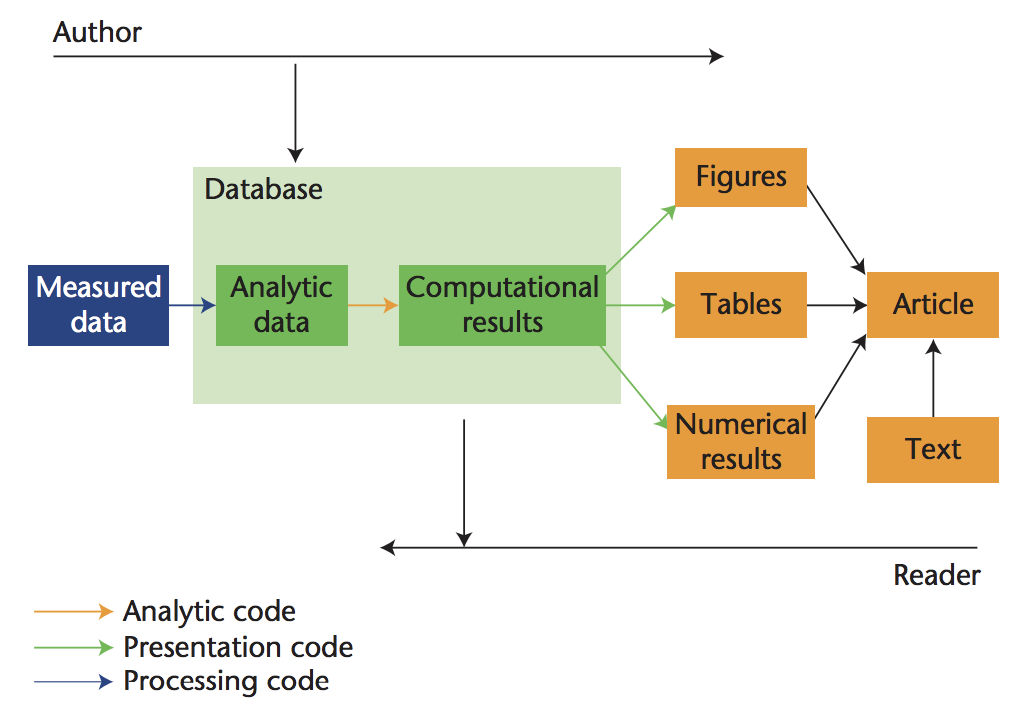
\includegraphics[width=9.5cm, keepaspectratio]{img/intro/rr_scheme.png}
\caption[RR generic scheme]{A scheme of Reproducible Research. (Image from \ref{Peng2009})}
\label{fig:omics}
\end{figure}

Because of the doubled complexity, due to the data analysis and to the time required to respect the \gls{rr} constraints, the \gls{rr} community always tried to provide tools to facilitate this process.
In particular, in bioinformatics community we can highlight the web platform Galaxy \cite{Aranguren2015, Goecks2010a} and the \textit{Bioconductor} community \cite{Gentleman2004, Shepherd2018}, which developers spend so much time and efforts to provide tools including a \gls{rr} layer.
But a standard has not been reached yet.

Unfortunately, despite all efforts of \gls{rr} community, the Life Science society is still far from a standard for reproducibility \cite{Iqbal2016}, showing that the way is still long to be covered.


